%----------------------------------------------------------------------------------------
%	TITLE PAGE
%----------------------------------------------------------------------------------------

\title{Study of Finite Temperature Kitaev Quantum Spin Liquid and Flux Energetics} % The short title appears at the bottom of every slide, the full title is only on the title page

\author{Kexin Feng\\
Advisors: Fiona Burnell, Natalia Perkins} % Your name
%\institute[UCLA] % Your institution as it will appear on the bottom of every slide, may be shorthand to save space
%{
%University of California \\ % Your institution for the title page
%\medskip
%\textit{john@smith.com} % Your email address
%}
\date{\today} % Date, can be changed to a custom date



\begin{frame}
    \titlepage % Print the title page as the first slide

%
\begin{figure}
    \begin{minipage}[c]{.25\textwidth}
        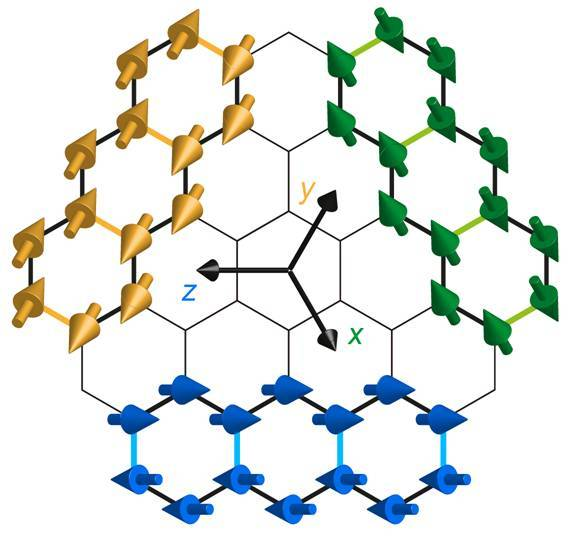
\includegraphics[width = 1\textwidth]{figures/Kim_manuscript_merged_F1.jpg} 
    \end{minipage}
    \hspace{2cm}
    \begin{minipage}[c]{.25\textwidth}
        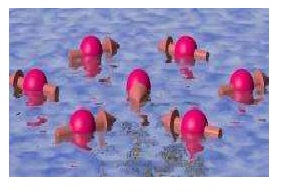
\includegraphics[width = 1\textwidth]{figures/quantummapma.jpg}
    \end{minipage}
\end{figure}
 
\end{frame}

\begin{frame}
    \frametitle{Overview} % Table of contents slide, comment this block out to remove it
    \tableofcontents % Throughout your presentation, if you choose to use \section{} and \subsection{} commands, these will automatically be printed on this slide as an overview of your presentation
\end{frame}